% Template for BiDS'19 papers; to be used with:
%          spconf.sty  - LaTeX style file, and
% --------------------------------------------------------------------------
\documentclass{article}
\usepackage{spconf,amsmath,epsfig}

\providecommand{\doi}[1]{doi: {\footnotesize \href{http://dx.doi.org/#1}{\path{#1}}}}

\usepackage[pdftex=true,breaklinks=true,hidelinks=true,colorlinks=true,citecolor=blue]{hyperref}
\usepackage{minted}
\setminted{fontsize=\tiny,baselinestretch=1}
\usepackage[square,numbers]{natbib}
\renewcommand{\bibsection}{\section*{\normalsize\hspace*{\fill}REFERENCES\hspace*{\fill}}}


% Example definitions.
% --------------------
\def\x{{\mathbf x}}
\def\L{{\cal L}}

% Title.
% ------
\title{The Pangeo Big Data Ecosystem and its use at CNES}
%
% Single address.
% ---------------
\name{Guillaume Eynard-Bontemps$^1$, Ryan Abernathey$^2$, Joseph Hamman$^3$, Aurelien Ponte$^4$, Willi Rath$^5$}%\thanks{Thanks to XYZ agency for funding.}}
\address{$^1$Centre National d'Etudes Spatiales (CNES), Toulouse, France,\\
$^2$Columbia University / Lamont Doherty Earth Observatory, New-York, USA,\\
$^3$National Center for Atmospheric Research (NCAR), Boulder, USA,\\
$^4$Ifremer, Univ. Brest, CNRS, IRD,  Laboratoire d’Océanographie Physique et Spatiale (LOPS), IUEM, Brest 29280, France,\\
$^5$GEOMAR Helmholtz Centre for Ocean Research Kiel, Kiel, Germany.}
%
% For example:
% ------------
%\address{School\\
%	Department\\
%	Address}
%
% Two addresses (uncomment and modify for two-address case).
% ----------------------------------------------------------
%\twoauthors
%  {A. Author-one, B. Author-two\sthanks{Thanks to XYZ agency for funding.}}
%	{School A-B\\
%	Department A-B\\
%	Address A-B}
%  {C. Author-three, D. Author-four\sthanks{The fourth author performed the work
%	while at ...}}
%	{School C-D\\
%	Department C-D\\
%	Address C-D}
%
\begin{document}
%\ninept
%
\maketitle
%
\begin{abstract}
Pangeo\cite{b1} is a community-driven effort for open-source big data initially
focused on the Earth System Sciences. One of its primary goals is to enable
scientists in analyzing peta-scale datasets both on classical high-performance
computing (HPC) and on public cloud infrastructure.  In only a few years, Pangeo
has grown into a very productive community collaborating on the development of
open-source analysis tools for science. 
It provides a set of example deployments based on open-source
Scientific Python packages like Jupyter\cite{b14}, Dask\cite{b12},
and Xarray\cite{b13} that bring together scientists and developer with their
actual use-cases.

In this paper, we first describe Pangeo ecosystem and community.
We then present its impact on the work of
scientists from CNES on the HPC deployment there.
We conclude with a future outlook for Pangeo in this agency and beyond.
\end{abstract}
%
\begin{keywords}
Pangeo, Dask, Jupyter, HPC, Cloud, Big Data, Analysis, Open Source
\end{keywords}
%
\section{Pangeo}
\label{sec:pangeo}

\subsection{Motivations}
\label{ssec:motivations}

The science community is facing several building crises: datasets are growing exponentially (see \ref{nasa_cloud_growth}) and legacy software tools for scientific analysis cannot handle them; a growing technology gap between the technological sophistication of industry solutions (high) and scientific software (low); the fragmentation of software tools and environments renders most science research effectively unreproducible and prone to failure.

\begin{figure}
  \centering
  \includegraphics[width=\columnwidth]{EOSDIS_archive_growth_updated_resize.jpg}
  \caption{\label{nasa_cloud_growth} Projected NASA EOS Cloud storage\cite{b2}.}
\end{figure}

Pangeo's core mission is to cultivate a collaborative environment in which the
next generation of open-source analysis tools for ocean, atmosphere, climate and
eventually other sciences can be developed, distributed, and sustained. These
tools must be scalable in order to meet the current and future challenges of big
data, and these solutions should leverage the existing expertise both inside and
outside of the geoscience community.

\subsection{Community}
\label{ssec:community}

Rather than being controlled by a single organization, Pangeo is a
community-driven project, in the model of successful open-source software like
Linux, Python, and Jupyter. In this spirit, all Pangeo discussions and products
occur on GitHub\cite{b3}, where anyone can easily get involved in the community.
As of today, Pangeo spans a list of people from different governmental agencies,
universities, or private companies, and from different countries (the USA, the
UK, France, Austalia to name a few). By making the collaboration as broad as
possible, Pangeo successfully leverages shared expertise to accomplish things no
institution could alone.


\subsection{Technology contributions to the Scientific Python stack}
\label{ssec:techstack}

Pangeo's software ecosystem fits directly into the Scientific Python stack, involving packages such as Numpy, Pandas, or Sickit-learn.  Three Python software projects are at the core of Pangeo:
\begin{itemize}
\item Dask is a library for parallel and distributed computing that coordinates with Python’s existing scientific software ecosystem. In many cases, it offers users the ability to take existing workflows and quickly scale them to much larger applications.
\item Xarray is the interface for working with big datasets: it provides a Pandas-like API for labelled n-dimensional arrays and has backends for established and upcoming self-describing community data file formats and access protocols like netCDF, GeoTIFF, OPeNDAP, and Zarr. Xarray transparently integrates Dask arrays and hence enables users to easily scale their work to massively parallel computations.
\item Jupyter: Jupyter notebooks and Jupyter Lab enable interactive computing and analysis from a web browser, and JupyterHub adds multi-user support. Jupyter notebooks are quickly becoming the standard open-source format for interactive computing not only in Python, but also in languages such as Julia and R.
\end{itemize}

\begin{figure}
  \centering
  \includegraphics[width=\columnwidth]{pangeo_stack.png}
  \caption{\label{pangeo_stack} Pangeo platform main components.}
\end{figure}

There are several developments that either started in or are fueled by the
Pangeo community. Modules to automatically deploy Dask distributed clusters in various infrastructures are being developed: dask-kubernetes for Kubernetes clusters and thus for the public cloud, dask-jobqueue\cite{b4} for HPC systems using scheduler such as Slurm, PBS Pro or LSF, and dask-yarn for YARN clusters (i.e. Hadoop).
The integration of a Zarr backend in Xarray paved the way to directly access cloud-based object storage in parallel computations.


\subsection{How Pangeo compares to other solutions}
\label{ssec:pangeoadvantages}

Pangeo primarily offers interactive or batch analysis of scientific datasets at scale. 
At the heart of this sentence are the three packages mentioned above: 
Jupyter for interactive, Dask for scale, Xarray (and Dask) for scientific 
datasets.
As such it can be compared to a lot of existing tools. We can think of 
\href{https://spark.apache.org/}{Apache Spark}, Rasdaman, SciDB, Myria,
or even more specific library like TensorFlow or 
\href{https://www.orfeo-toolbox.org/}{Orfeo ToolBox (OTB)}. First ones are
already mentioned in a paper about imagery analysis \cite{b4_2} (where they
are compared to Dask only).

Pangeo is not another Datacube or scientific database, but you can
build one using its core packages, as the 
\href{https://www.opendatacube.org}{Open Data Cube} team is doing. Xarray
backed by Dask allows powerful and at scale complex data manipulation such as
regridding, datasets fusion and so one. Another example shows how to perform some 
\href{https://earthengine.google.com/}{Google Earth Engine} like
analysis using Pangeo \cite{b6}.

Dask can be compared to Spark, but is more versatile: it does not only
handles big collections or SQL like queries, it can also perform distributed
nd-arrays operations, or any kind of inter node multiprocessing workload using
Delayed or Future API. There has been some experiment to use Spark for Dask/Xarray like analysis with
\href{https://scispark.jpl.nasa.gov/}{NASA SciSpark}, but it was not really
conclusive.

Dask and Xarray can be leveraged interactively from a Jupyter notebook plugged to
a compute infrastructure (e.g. HPC or Kubernetes cluster in the Cloud). A user
can make use of the computing power with two or three lines of code and perform
manipulation on tens of Terabytes of data as if handling some Megabytes on its
own laptop.

Pangeo is not a focused scientific library such as OTB or TensorFlow.
It provides more high level means to use these domain specific modules: 
it could be used to provide some ways to orchestrate complex OTB applications,
or launch them at scale over thousand of images. It could also be used to prepare 
data before feeding it to TensorFlow or other Deep Learning libraries.


\subsection{Deployment}
\label{ssec:deployment}

The GitHub community offers online documentation, scripts and other tools to link them together in order to deploy a Pangeo platform (see \ref{pangeo_stack}) and put the software stack on HPC systems or in the public cloud. The main elements allowing to build and use the platform in the cloud are a set of scripts and documentation that allows automatically creating the necessary cloud infrastructure (a Kubernetes autoscaling cluster), a Helm-chart and associated Docker image, which heavily relies on Jupyterhub solutions. This is currently available for Google Cloud Engine (GCE), and work is underway for Amazon Web Services (AWS) compatibility. Continuous Deployment tooling is also used for automating new Pangeo versions deployment with Hubploy and CircleCI. To facilitate learning and using the Pangeo software stack at scale, there is a Binder deployment\cite{b8} enabling the live execution of any compatible github repo (providing environment description and some example notebooks) in a single click, on Pangeo existing Google cloud infrastructure.


\subsection{Applications and data}
\label{ssec:applications}

There are already several applications documented in earth-system sciences that can be found online\cite{b5}; these examples can be directly executed on cloud infrastructure from a web browser, associated datasets are also published on Pangeo public bucket in a Cloud friendly format. 
Other scientific domains have developed an interest in the Pangeo approach, including Satellite imagery analysis \cite{b6}, Astronomy or Neuroscience.

As the computational resources necessary for most of these applications can only
be met with distributed computing, the data must be in a cloud or distributed
storage friendly format, like Zarr for multi-dimensional data, Cloud optimized
Geotiff for satellite imagery, or Parquet for tabular data. See \cite{b7} and
\cite{b11} for more details on this crucial point.


\section{CNES deployment and use cases}
\label{sec:cnes}

\subsection{Context and projects}
\label{ssec:context}

The Centre National d'Etudes Spatiales (CNES) is the government agency responsible for shaping and implementing France's space policy in Europe. As such it covers a wide range of subjects: Ariane launcher, Sciences, Earth observation, telecommunication and defence.

On the ground segment processing side, we are involved in several Big Data projects, most of them being hosted in CNES Data Center: one of the Gaia data processing center; Sentinel product Exploitation Platform, for sharing and online processing of Copernicus products; Surface Water and Ocean Topography (SWOT) mission...

CNES HPC platform is also hosting a lot of other processing involving remote sensing data, flight dynamics, altimetry or other domains.

\subsection{Pangeo on our HPC System}
\label{ssec:pangeohpc}

\begin{figure}
  \centering
  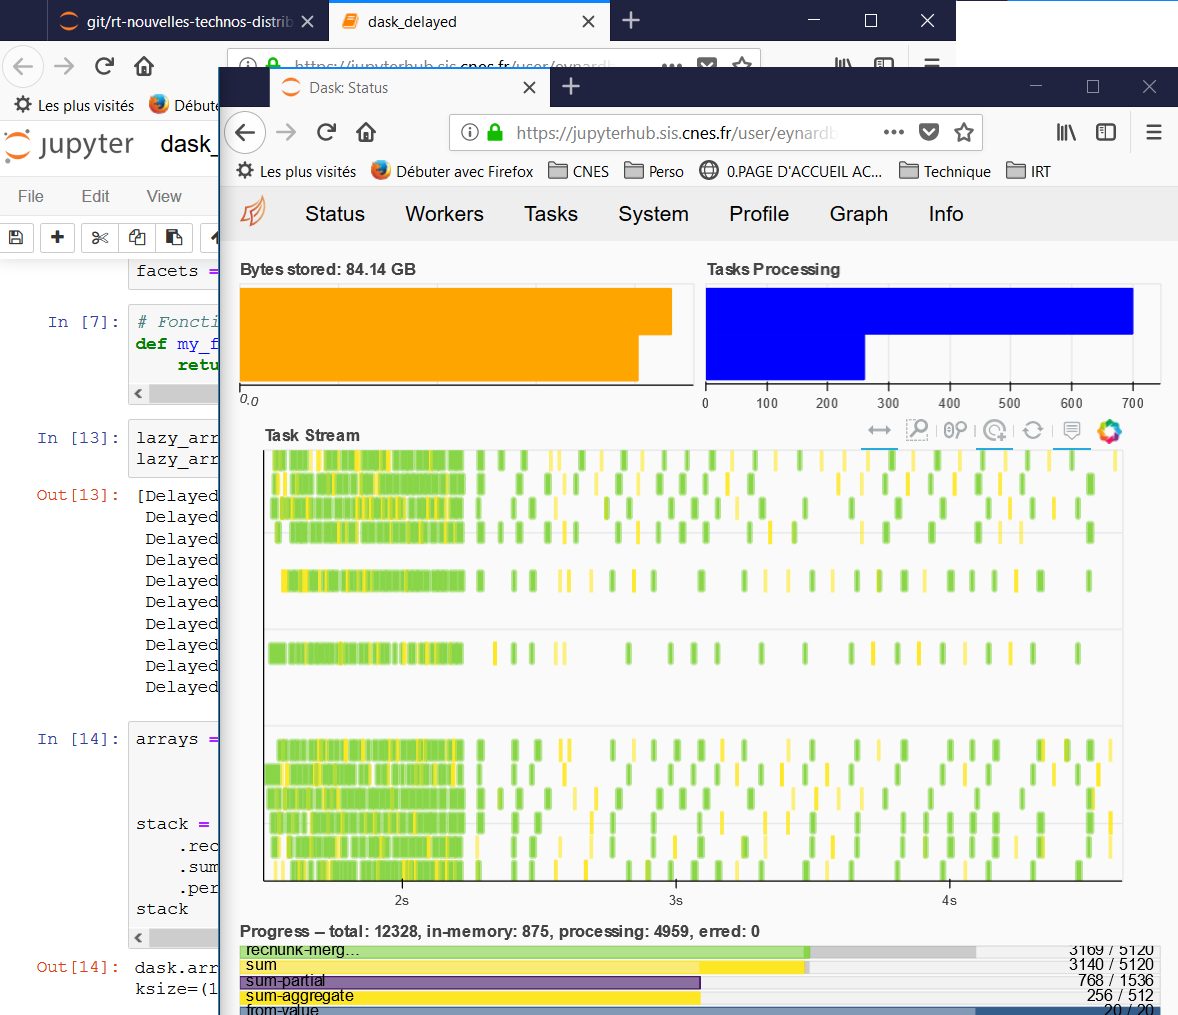
\includegraphics[width=\columnwidth]{dask_jobqueue.png}
  \caption{\label{dask_jobqueue} Computation in Jupyter and Dask dashboard.}
\end{figure}

CNES main processing platform is a modestly sized High Performance Computer named HAL. Its computational resources are about 8000 Intel cores and 6PB high bandwidth storage. It uses PBS Pro jobqueue system to schedule the load on compute nodes and handle user and project resource sharing.

Pangeo platform has recently been deployed on the cluster, which basically means the configuration of two main components: a JupyterHub, and Dask through dask-jobqueue (see \ref{dask_jobqueue} for a graphical overview). JupyterHub has been deployed on a Virtual Machine, which has direct access to HAL cluster through PBS commands. This allows configuring JupyterHub Batchspawner which launches user notebooks using PBS \textit{qsub} command, alongside Wrapspwaner to be able to select adequate system resources for launched notebook.

CNES directly contributes to dask-jobqueue in order to improve its usability on HAL. This Python module deployment (alike Xarray or other domain scientific library) is quite simple as it can be done through conda or pip packaging system. All of this is documented, and some demonstration notebooks have been shared internally.

\subsection{From embarrassingly parallel to more complex workflows with Dask}
\label{ssec:usecase1}

\begin{figure}
\begin{minted}[linenos,
               frame=lines,
               framesep=2mm,
               fontsize=\small]{python}
# Create cluster and scale to 8 nodes
from dask_jobqueue import PBSCluster
cluster = PBSCluster(cores=24, memory="120GB", 
                     interface='ib0')
cluster.scale(8)

# Connect to cluster
from dask.distributed import Client
client = Client(cluster)

# Submit a function on a list of inputs
futures = client.map(my_costly_simulation, 
                     input_params)
results = client.gather(futures)

# Compute and plot the mean on time series
df[['x', 'y']].resample('2w').mean()
              .compute().plot()
\end{minted}
\caption{\label{ep_dask_code} Embarrassingly parallel workload using Dask.}
\end{figure}

One important use of our cluster is to do repetitive jobs: apply the same computation or process to several inputs, which can for example be a list of files or a list of parameters. This is usually done with job arrays PBS mechanism. Results are then written into our central storage facility, and a final job gathers and consolidates them if needed. There are three main drawbacks to this approach:
\begin{itemize}
\item When scaling this mechanism to hundreds of thousands and short (under one minute) jobs, this can lead to PBS scheduler contention and slow responsiveness.
\item This often means a lot of bash script and machinery to chain several analysis together, leading to workflows that are hardly readable and difficult to maintain.
\item As results can be really small and are exchanged through a centralized storage system, this also means a lot of I/O load onto the File System and side effects for other users.
\end{itemize}

Pangeo, mainly through Dask, gives an adequate solution to all these problems (see \ref{ep_dask_code} for an example). All the workflow, cluster creation, data management parts are handled from Python code. Reservation to PBS are done using dask-mpi or dask-jobqueue. No need to write or exchange data through disk, all data management is done through memory or network with TCP over high-speed networks (i.e. Infiniband). This allows users to analyze the result of a simulation in the same piece of code where it has been launched, and eventually gather only the reduced valuable part for later use. The result of all this is elegant and simple Python code, which can scale easily to thousands of cores and does not stress our HPC cluster.

\subsection{Surface ocean currents analysis at scale}
\label{ssec:usecase3}

Ifremer (Institut français de recherche pour l'exploitation de la mer) used CNES
Pangeo provided tooling to develop and run one of 
\href{https://github.com/apatlpo/mit_equinox/blob/master/hal/rechunk_rotspectra.ipynb}{their workflow}. Ifremer already used Dask before\cite{b9}.

Surface ocean currents from a global high resolution numerical simulation are analyzed in order to compute time-frequency kinetic energy spectra.
Spectra are averaged zonally in order to emphasize meridional variations of these spectra.
These spectra may be compared to observed estimates in order to validate the numerical model for example.
The input data consists of a collection of snapshots which is a layout that does not allow computations that are global in time such as an \textit{fft}.
The analysis thus starts with a rechunking of the data into larger temporal chunks and smaller spatial ones.
Spectra are then computed and averaged in latitude bins.
Each of the latter stage leverage the distribution of existing sequential \textit{fft} code to Xarray objects via the \textit{apply_ufunc} method.


\section{Conclusion}
\label{sec:conclusion}

Pangeo is a powerful ecosystem which enables science at scale on Cloud or on premise infrastructure. We encourage every lab, government agency, or even industry players to take a look at what it provides. The community is open and eager to welcome new users and collaborators.
At CNES, we decided to focus on this tooling for our shared computing infrastructure, and it is already showing its power and its benefit. Ongoing work is focusing on developing more and more use cases with Pangeo to identify where it is most useful, and possible limits to the software stack. We are also trying to participate actively in the community and share our vision and needs, helping to steer the common effort in a direction beneficial to CNES researchers.

% To start a new column (but not a new page) and help balance the last-page
% column length use \vfill\pagebreak.
% -------------------------------------------------------------------------
%\vfill
%\pagebreak


% References should be produced using the bibtex program from suitable
% BiBTeX files
% -------------------------------------------------------------------------

\bibliographystyle{plainnat}
\bibliography{myBibFile}

\small

\begin{thebibliography}{00}
\bibitem{b1} Ryan Abernathey, Kevin Paul, Joseph Hamman, Matthew Rocklin, Chiara Lepore, Michaem Tippett, et al. (2017): \href{https://figshare.com/articles/Pangeo_NSF_Earthcube_Proposal/5361094}{Pangeo NSF Earthcube Proposal}.
\bibitem{b14} Thomas Kluyver et al: Jupyter notebooks -- a publishing format for reproducible computational workflows. In F.~Loizides and B.~Schmidt, editors, \emph{Positioning and Power in Academic Publishing: Players, Agents and Agendas}, pages 87 -- 90. IOS Press, 2016.
\bibitem{b12} Dask Development Team: \href{https://dask.org}{Dask: Library for dynamic task scheduling}, 2016.
\bibitem{b13} Stephan Hoyer and Joseph~J. Hamman: xarray: N-d labeled arrays and datasets in python. \emph{Journal of Open Research Software}, 5, apr 2017. \doi{10.5334/jors.148}.
\bibitem{b2} Mark McInerney, ESDIS Project Deputy Project Manager/Technical: EOSDIS Cloud Evolution\href{https://earthdata.nasa.gov/about/eosdis-cloud-evolution}{NASA EOSDIS web site}.
\bibitem{b3} Ryan Abernathey et al: \href{https://github.com/pangeo-data/pangeo/issues}{Pangeo github project issue tracker}.
\bibitem{b4} Joseph Hamman, Matthew Rocklin, Jim Edwards, Guillaume Eynard-Bontemps, Loic Esteve (2018): \href{https://medium.com/pangeo/dask-jobqueue-d7754e42ca53}{Scalable interactive analysis workflows using dask on HPC Systems}.
\bibitem{b4_2} Parmita Mehta et al (2016): \href{https://arxiv.org/abs/1612.02485}{Comparative Evaluation of Big-Data Systems on Scientific Image Analytics Workloads}.
\bibitem{b6} Scott Henderson, Daniel Rothenberg, Matthew Rocklin, Ryan Abernathey, Joseph Hamman, Rich Signell, and Rob Fatland: \href{https://medium.com/pangeo/cloud-native-geoprocessing-of-earth-observation-satellite-data-with-pangeo-997692d91ca2}{Cloud Native Geoprocessing of Earth Observation Satellite Data with Pangeo}.
\bibitem{b8} Joseph Hamman, Ryan Abernathey: \href{https://medium.com/pangeo/pangeo-meets-binder-2ea923feb34f}{Pangeo meets Binder}.
\bibitem{b5} Pangeo community: \href{http://pangeo.io/use_cases/index.html}{Pangeo use cases}.
\bibitem{b7} Ryan Abernathey: \href{https://medium.com/pangeo/step-by-step-guide-to-building-a-big-data-portal-e262af1c2977}{Step-by-Step Guide to Building a Big Data Portal}.
\bibitem{b11} Matthew Rocklin: \href{https://matthewrocklin.com/blog/work/2018/02/06/hdf-in-the-cloud}{HDF in the Cloud --- Challenges and solutions for scientific data}. \doi{10.3233/978-1-61499-649-1-87}.
\bibitem{b9} S. Fresnay, A. L. Ponte, S. Le Gentil, and J. Le Sommer: Reconstruction of the 3-D Dynamics From Surface Variables in
a High-Resolution Simulation of North Atlantic. \href{https://agupubs.onlinelibrary.wiley.com/doi/abs/10.1002/2017JC013400}{DOI: 10.1002/2017JC013400}.
\bibitem{b10} Joe Hamman: \href{https://medium.com/pangeo/nasa-access-c3515a44f31b}{Pangeo applications for NASA Earth Observing Data}.
\end{thebibliography}
\end{document}
